
\section{Results}
\label{sec:results}


We present the results according to the research questions defined in Section ~\ref{sec:research-questions}.

\subsection{RQ1: How can energy consumption of small code blocks be measured accurately and reproducibly?}

\begin{figure}[t]
  \centering
  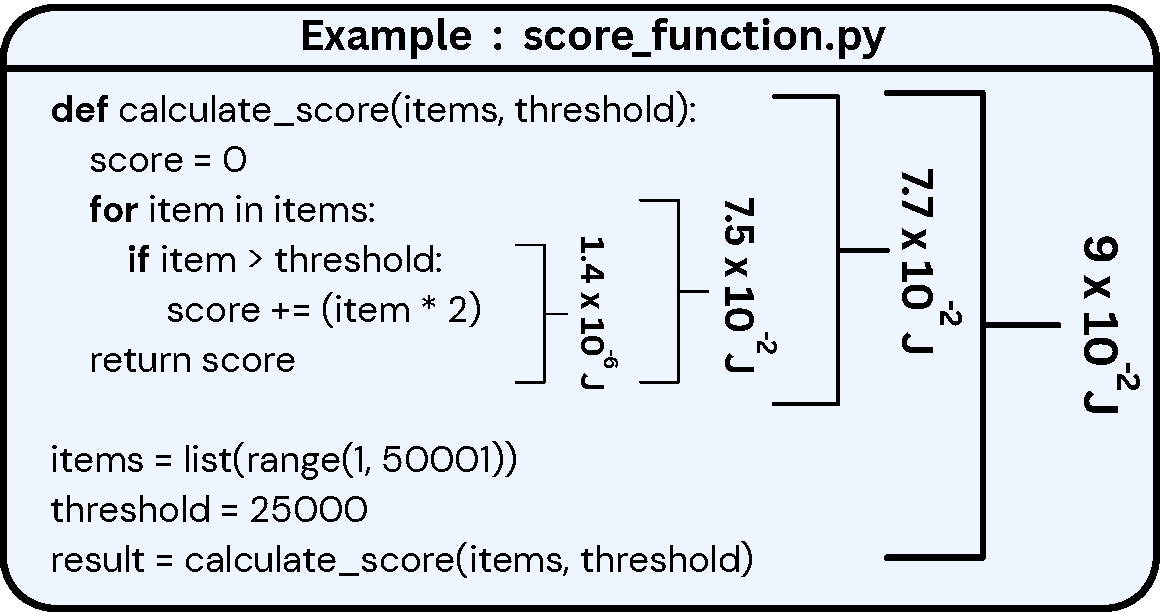
\includegraphics[width=1\linewidth]{figures/example_measurement.pdf}
  \caption{Block Level Energy Measurement of the score computation function}
  \label{fig:example-measurement}
\end{figure}
Our first research question examines whether energy consumption of microsecond-scale code blocks can be measured accurately and reproducibly.  Each block was measured ten times, and across the dataset \textbf{more than 90\%} of the blocks exhibited \textbf{less than 10\% variation} between repeated trials after IQR outlier removal, indicating strong measurement stability and effective suppression of environmental noise. The results demonstrate that the proposed measurement infrastructure provides stable and reliable energy values at block granularity. This is a result of system stabilization and calibrated padding loops.

The measurement protocol also achieves both high sensitivity and broad coverage. The observed energy values spans six orders of magnitude, ranging from $2.37 \times 10^{-5}$ joules for trivial blocks to $7.48 \times 10^{2}$ joules for complex functions. This wide dynamic range confirms that the methodology is capable of capturing energy signatures of extremely short-lived constructs while remaining reliable. Without the amplification and synchronization mechanisms, many of these fine-grained blocks would register highly unstable or zero readings using conventional software-profilers.

Figure~\ref{fig:example-measurement} illustrates block-level energy measurements for the \texttt{score\_function.py} example, where annotated values indicate per-block energy consumption in joules as measured by PowerLens in Nested Blocks.
Figure~\ref{fig:powerlens-pyrapl} compares the sum of block-level energy measurements obtained with PowerLens against coarse-grained measurements from PyRAPL\footnote{\url{https://github.com/powerapi-ng/pyRAPL}}, grouped by construct type. To \textbf{validate} the correctness of the fine-grained measurements, we compared the aggregate energy obtained by summing block-level measurements from PowerLens with the total program-level energy reported by PyRAPL for the same codes, across 40 instances of each block type (see Figure~\ref{fig:powerlens-pyrapl}). For all block categories, the aggregated PowerLens measurements closely match the corresponding coarse-grained energy reported by PyRAPL. In addition, PowerLens exhibits \textbf{substantially lower variance} across repeated measurements, as it stabilizes the execution environment and applies calibration loops to isolate block execution energy.
% These results confirm that \textbf{PowerLens} provides \textbf{reliable, high-resolution} energy measurements across diverse code constructs while remaining consistent with established coarse-grained profiling tools.


\begin{rqbox}{Answer to RQ1}Together, these results confirm that PowerLens enables accurate, stable, and reproducible energy measurement at the level of individual small code blocks, overcoming the temporal limitations of existing software-based profilers.
\end{rqbox}

\begin{figure}[t]
  \centering
  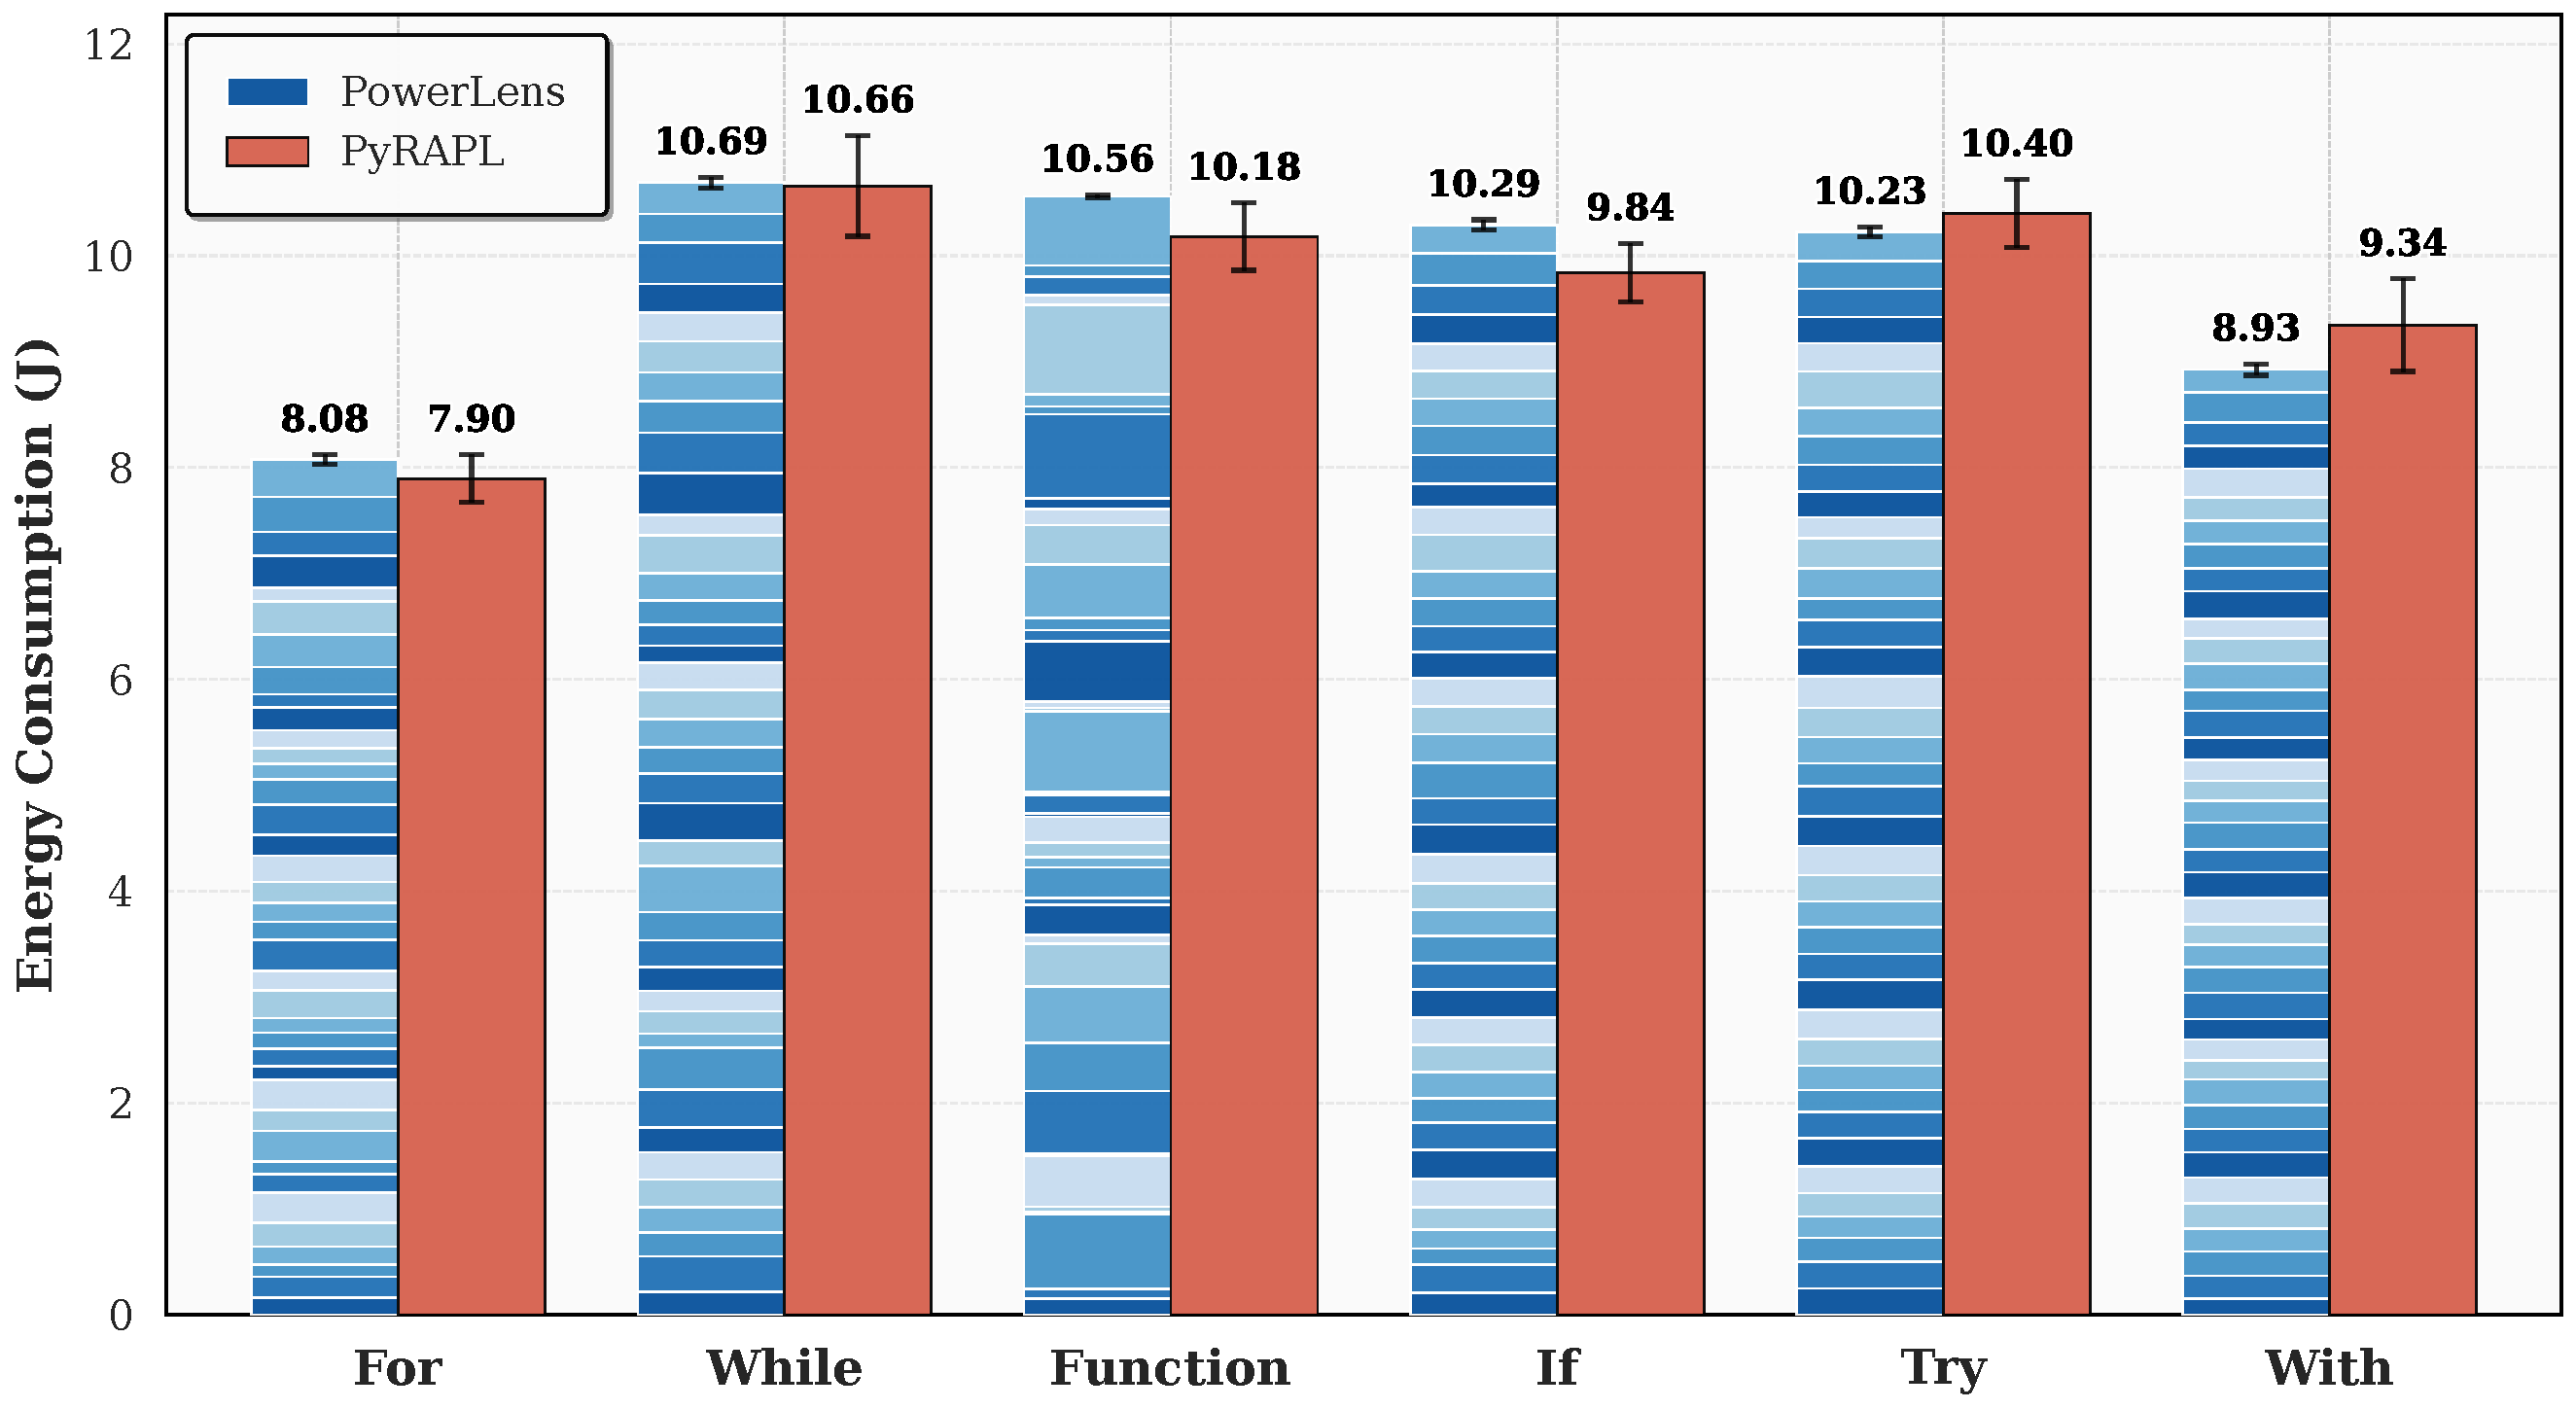
\includegraphics[width=1\linewidth]{figures/validation_plot_hq.pdf}
  \caption{Sum of Blocks measured by Powerlens compared with Overall measurement by Pyrapl}
  \label{fig:powerlens-pyrapl}
\end{figure}
% \textbf{\textit{PLACEHOLDER: Boxplot of measurement variance across blocks; histogram of block-level energy distribution.}}

\subsection{RQ2: What statistical relationships exist between static code features and block-level energy consumption?}


% \begin{table*}[htbp]
% \centering
% \caption{Top 20 features ranked by correlation and model-based importance methods.}
% \resizebox{\textwidth}{!}{%
% \begin{tabular}{c l c l c l c l c l c l c}
% \hline
% Rank & \multicolumn{2}{c}{Pearson ($r$)} & \multicolumn{2}{c}{Spearman ($\rho$)} & 
% \multicolumn{2}{c}{Kendall ($\tau$)} & \multicolumn{2}{c}{Gradient Boost} & \multicolumn{2}{c}{XGBoost} & \multicolumn{2}{c}{Random Forest}\\
% \cline{2-13}
% & Feature & Value & Feature & Value & Feature & Value & Feature & Value & Feature & Value & Feature & Value\\
% \hline
% 1    & \cellcolor[HTML]{A0C3D5}functions count      & 0.704  & \cellcolor[HTML]{A0C3D5}functions count      & 0.616 & \cellcolor[HTML]{A0C3D5}functions count      & 0.503 & \cellcolor[HTML]{A0C3D5}functions count       & 0.620 & \cellcolor[HTML]{A0C3D5}functions count       & 0.410 & \cellcolor[HTML]{A0C3D5}functions count         & 0.273 \\
% 2    & \cellcolor[HTML]{A0C3D5}node type entropy    & 0.434  & \cellcolor[HTML]{A0C3D5}node type entropy    & 0.393 & \cellcolor[HTML]{A0C3D5}node type entropy    & 0.263 & \cellcolor[HTML]{F8CBAD}depth variance        & 0.140 & \cellcolor[HTML]{D4E7C5 }leaves to nodes ratio & 0.062 & \cellcolor[HTML]{A0C3D5}node type entropy       & 0.097 \\
% 3    & \cellcolor[HTML]{A0C3D5}unique node types    & 0.372  & \cellcolor[HTML]{A0C3D5}unique node types    & 0.347 & \cellcolor[HTML]{A0C3D5}unique node types    & 0.243 & \cellcolor[HTML]{D4E7C5 }leaves to nodes ratio & 0.096 & \cellcolor[HTML]{D4E7C5 }call density          & 0.061 & \cellcolor[HTML]{A0C3D5}unique node types       & 0.064 \\
% 4    & \cellcolor[HTML]{F8CBAD}depth variance       & 0.222  & \cellcolor[HTML]{F8CBAD}depth variance       & 0.326 & \cellcolor[HTML]{F8CBAD}max branching factor & 0.243 & \cellcolor[HTML]{D4E7C5 }call density          & 0.087 & \cellcolor[HTML]{A0C3D5}node type entropy     & 0.057 & \cellcolor[HTML]{D4E7C5 }leaves to nodes ratio   & 0.035 \\
% 5    & \cellcolor[HTML]{F8CBAD}max branching factor & 0.218  & \cellcolor[HTML]{F8CBAD}max branching factor & 0.317 & \cellcolor[HTML]{F8CBAD}depth variance       & 0.220 & \cellcolor[HTML]{F8CBAD}variable density      & 0.075 & \cellcolor[HTML]{F8CBAD}depth variance        & 0.049 & \cellcolor[HTML]{F8CBAD}depth variance          & 0.035 \\
% 6    & max depth                                    & 0.192  & max depth                                    & 0.281 & max depth                                    & 0.206 & \cellcolor[HTML]{D4E7C5 }avg depth             & 0.067 & \cellcolor[HTML]{F8CBAD}variable density      & 0.040 & \cellcolor[HTML]{D4E7C5 }cyclomatic complexity   & 0.034 \\
% 7    & \cellcolor[HTML]{D4E7C5 }avg depth            & 0.137  & \cellcolor[HTML]{D4E7C5 }avg depth            & 0.221 & \cellcolor[HTML]{D4E7C5 }avg depth            & 0.148 & \cellcolor[HTML]{A0C3D5}node type entropy     & 0.067 & \cellcolor[HTML]{A0C3D5}unique node types     & 0.037 & \cellcolor[HTML]{D4E7C5 }call density            & 0.033 \\
% 8    & \cellcolor[HTML]{D4E7C5 }total nodes          & 0.114  & \cellcolor[HTML]{D4E7C5 }total nodes          & 0.181 & unique functions                             & 0.126 & \cellcolor[HTML]{D4E7C5 }operator density      & 0.050 & \cellcolor[HTML]{D4E7C5 }avg depth             & 0.035 & \cellcolor[HTML]{D4E7C5 }control flow complexity & 0.032 \\
% 9    & program volume                               & 0.075  & \cellcolor[HTML]{D4E7C5 }avg branching factor & 0.181 & \cellcolor[HTML]{D4E7C5 }total nodes          & 0.125 & \cellcolor[HTML]{D4E7C5 }attribute density     & 0.047 & \cellcolor[HTML]{F8CBAD}max branching factor  & 0.034 & \cellcolor[HTML]{D4E7C5 }cognitive complexity    & 0.032 \\
% 10   & \cellcolor[HTML]{D4E7C5 }avg branching factor & 0.073  & unique functions                             & 0.156 & \cellcolor[HTML]{D4E7C5 }avg branching factor & 0.125 & \cellcolor[HTML]{D4E7C5 }literal density       & 0.031 & \cellcolor[HTML]{D4E7C5 }cognitive complexity  & 0.022 & \cellcolor[HTML]{F8CBAD}max branching factor    & 0.031 \\
% 11   & program length                               & 0.073  & vocabulary size                              & 0.142 & vocabulary size                              & 0.104 & \cellcolor[HTML]{A0C3D5}unique node types     & 0.026 & \cellcolor[HTML]{D4E7C5 }operator density      & 0.022 & \cellcolor[HTML]{F8CBAD}variable density        & 0.030 \\
% 12   & unique operators                             & 0.070  & program volume                               & 0.136 & program volume                               & 0.095 & \cellcolor[HTML]{F8CBAD}max branching factor  & 0.022 & \cellcolor[HTML]{D4E7C5 }cyclomatic complexity & 0.018 & \cellcolor[HTML]{D4E7C5 }operator density        & 0.029 \\
% 13   & operator entropy                             & 0.067  & program length                               & 0.128 & loops count                                  & 0.092 & variable entropy                              & 0.018 & \cellcolor[HTML]{D4E7C5 }literal density       & 0.017 & \cellcolor[HTML]{D4E7C5 }nesting complexity      & 0.025 \\
% 14   & program difficulty                           & 0.061  & unique variables                             & 0.114 & program length                               & 0.091 & \cellcolor[HTML]{D4E7C5 }nesting complexity    & 0.017 & \cellcolor[HTML]{D4E7C5 }attribute density     & 0.016 & \cellcolor[HTML]{D4E7C5 }avg depth               & 0.025 \\
% 15   & vocabulary size                              & 0.052  & variable entropy                             & 0.112 & unique variables                             & 0.090 & program difficulty                            & 0.016 & variable entropy                              & 0.014 & \cellcolor[HTML]{D4E7C5 }literal density         & 0.021 \\
% 16   & program effort                               & 0.051  & loops count                                  & 0.110 & variable entropy                             & 0.083 & \cellcolor[HTML]{D4E7C5 }total nodes           & 0.015 & \cellcolor[HTML]{D4E7C5 }total nodes           & 0.014 & \cellcolor[HTML]{D4E7C5 }total nodes             & 0.020 \\
% 17   & \cellcolor[HTML]{D4E7C5 }operator density     & 0.018  & program effort                               & 0.068 & program effort                               & 0.048 & conditionals count                            & 0.012 & \cellcolor[HTML]{D4E7C5 }nesting complexity    & 0.013 & \cellcolor[HTML]{D4E7C5 }avg branching factor    & 0.020 \\
% 18   & \cellcolor[HTML]{D4E7C5 }attribute density    & 0.012  & \cellcolor[HTML]{D4E7C5 }literal density      & 0.047 & operator entropy                             & 0.032 & \cellcolor[HTML]{D4E7C5 }cyclomatic complexity & 0.011 & unique functions                              & 0.011 & \cellcolor[HTML]{D4E7C5 }attribute density       & 0.017 \\
% 19   & unique variables                             & 0.008  & operator entropy                             & 0.043 & \cellcolor[HTML]{D4E7C5 }literal density      & 0.031 & program effort                                & 0.010 & program difficulty                            & 0.011 & variable entropy                                & 0.017 \\
% 20   & try blocks count                             & -0.004 & unique operators                             & 0.022 & unique operators                             & 0.015 & unique functions                              & 0.008 & \cellcolor[HTML]{D4E7C5 }avg branching factor  & 0.010 & program difficulty                              & 0.016 \\
% \hli 0ne
% \end{tabular}
% }
% \label{tab:feature_ranking}
% \end{table*}
% \begin{table*}[htbp]
% \centering
% \caption{Top 20 features by Correlation and Feature Importance}
% \resizebox{\textwidth}{!}{%
% \begin{tabular}{c l c l c l c l c l c}
% \hline
% Rank & \multicolumn{2}{c}{Pearson ($r$)} & \multicolumn{2}{c}{Spearman ($\rho$)} & 
% \multicolumn{2}{c}{Kendall ($\tau$)} & \multicolumn{2}{c}{ExtraTrees} & \multicolumn{2}{c}{Random Forest}\\
% \cline{2-11}
% & Feature & Value & Feature & Value & Feature & Value & Feature & Value & Feature & Value\\
% \hline
% 1    & \cellcolor[HTML]{FDB462}operator density          & 0.176  & unique functions                      & 0.392 & unique functions                      & 0.305 & \cellcolor[HTML]{FDB462}call density          & 0.137 & \cellcolor[HTML]{FDB462}call density          & 0.299 \\
% 2    & operator entropy                                  & 0.139  & vocabulary size                       & 0.319 & unique variables                      & 0.230 & \cellcolor[HTML]{FDB462}operator density      & 0.069 & \cellcolor[HTML]{FDB462}program difficulty    & 0.174 \\
% 3    & \cellcolor[HTML]{FDB462}literal density           & 0.122  & unique variables                      & 0.301 & vocabulary size                       & 0.227 & \cellcolor[HTML]{FDB462}depth variance        & 0.065 & \cellcolor[HTML]{FDB462}operator density      & 0.126 \\
% 4    & unique operators                                  & 0.122  & \cellcolor[HTML]{FDB462}variable entropy                      & 0.291 & loops count                           & 0.223 & \cellcolor[HTML]{FDB462}literal density       & 0.061 & \cellcolor[HTML]{FDB462}variable entropy                      & 0.062 \\
% 5    & conditionals count                                & 0.114  & \cellcolor[HTML]{FDB462}call density          & 0.281 & \cellcolor[HTML]{FDB462}variable entropy                      & 0.210 & \cellcolor[HTML]{FDB462}variable entropy                      & 0.059 & \cellcolor[HTML]{FDB462}node type entropy     & 0.038 \\
% 6    & variable density                                  & 0.099  & program volume                        & 0.274 & \cellcolor[HTML]{FDB462}call density          & 0.199 & unique node types     & 0.042 & \cellcolor[HTML]{FDB462}depth variance        & 0.031 \\
% 7    & \cellcolor[HTML]{FDB462}program difficulty        & 0.093  & loops count                           & 0.271 & max depth                             & 0.192 & leaves to nodes ratio & 0.041 & program effort                        & 0.026 \\
% 8    & loops count                                       & 0.092  & max depth                             & 0.258 & program volume                        & 0.188 & variable density                      & 0.041 & unique node types     & 0.023 \\
% 9    & \cellcolor[HTML]{FDB462}depth variance            & 0.091  & program length                        & 0.247 & cognitive complexity  & 0.173 & operator entropy                      & 0.040 & variable density                      & 0.021 \\
% 10   & \cellcolor[HTML]{FDB462}variable entropy                                  & 0.084  & \cellcolor[HTML]{FDB462}depth variance        & 0.247 & program length                        & 0.173 & avg depth             & 0.040 & \cellcolor[HTML]{FDB462}literal density       & 0.018 \\
% 11   & functions count           & 0.077  & avg depth             & 0.237 & control flow complexity & 0.168 & \cellcolor[HTML]{FDB462}program difficulty    & 0.038 & program length                        & 0.017 \\
% 12   & unique variables                                  & 0.069  & cognitive complexity  & 0.226 & \cellcolor[HTML]{FDB462}depth variance        & 0.168 & unique functions                      & 0.037 & avg depth             & 0.017 \\
% 13   & leaves to nodes ratio     & 0.062  & total nodes           & 0.224 & nesting complexity    & 0.168 & \cellcolor[HTML]{FDB462}node type entropy     & 0.032 & leaves to nodes ratio & 0.016 \\
% 14   & avg depth                 & 0.062  & avg branching factor  & 0.224 & cyclomatic complexity & 0.168 & max depth                             & 0.030 & max depth                             & 0.015 \\
% 15   & max depth                                         & 0.061  & cyclomatic complexity & 0.218 & max branching factor  & 0.164 & vocabulary size                       & 0.030 & vocabulary size                       & 0.014 \\
% 16   & attribute density         & 0.056  & control flow complexity & 0.217 & avg depth             & 0.163 & unique variables                      & 0.027 & unique functions                      & 0.012 \\
% 17   & \cellcolor[HTML]{FDB462}node type entropy         & 0.045  & nesting complexity    & 0.217 & total nodes           & 0.157 & loops count                           & 0.023 & unique variables                      & 0.012 \\
% 18   & cognitive complexity      & 0.039  & max branching factor  & 0.210 & avg branching factor  & 0.157 & unique operators                      & 0.022 & program volume                        & 0.012 \\
% 19   & nesting complexity        & 0.034  & \cellcolor[HTML]{FDB462}literal density       & 0.183 & \cellcolor[HTML]{FDB462}literal density       & 0.128 & program volume                        & 0.021 & total nodes           & 0.012 \\
% 20   & avg branching factor      & 0.034  & unique node types     & 0.134 & unique node types     & 0.094 & avg branching factor  & 0.021 & avg branching factor  & 0.011 \\
% \hline
% \end{tabular}
% }
% \label{tab:feature_ranking}
% \end{table*}


\begin{table*}[htbp]
\centering
\caption{Top 20 features by Correlation and Feature Importance}
\resizebox{\textwidth}{!}{%
\begin{tabular}{lllllllllllll}
\hline
Rank & \multicolumn{2}{l}{Pearson ($|r|$)}          & \multicolumn{2}{l}{Spearman ($|\rho|$)}      & \multicolumn{2}{l}{Kendall (|$\tau$|)}       & \multicolumn{2}{l}{ExtraTrees}               & \multicolumn{2}{l}{Random Forest}            & \multicolumn{2}{l}{Gradient Boosting}        \\ \cline{2-13} 
     & Feature                     & Value          & Feature                     & Value          & Feature                     & Value          & Feature                     & Value          & Feature                     & Value          & Feature                     & Value          \\ \hline
1    & \textbf{operator density}   & \textbf{0.286} & \textit{functions count}    & \textit{0.621} & \textit{functions count}    & \textit{0.507} & \textbf{operator density}   & \textbf{0.086} & \textbf{operator density}   & \textbf{0.099} & \textbf{operator density}   & \textbf{0.102} \\
2    & \textbf{operator entropy}   & \textbf{0.205} & node type entropy           & 0.294          & node type entropy           & 0.193          & \textbf{loops count}        & \textbf{0.063} & \textit{unique node types}  & \textit{0.075} & \textbf{program difficulty} & \textbf{0.056} \\
3    & conditionals count          & 0.181          & \textit{conditionals count} & \textit{0.229} & \textit{conditionals count} & \textit{0.178} & \textit{functions count}    & \textit{0.061} & \textbf{program difficulty} & \textbf{0.073} & program effort              & 0.054          \\
4    & unique operators            & 0.178          & cognitive complexity        & 0.225          & cognitive complexity        & 0.165          & \textbf{operator entropy}   & \textbf{0.054} & \textit{call density}       & \textit{0.072} & \textit{variable entropy}   & \textit{0.037} \\
5    & \textit{literal density}    & \textit{0.174} & nesting complexity          & 0.215          & unique functions            & 0.165          & \textit{variable entropy}   & \textit{0.054} & \textit{variable entropy}   & \textit{0.061} & \textbf{loops count}        & \textbf{0.037} \\
6    & functions count             & 0.166          & control flow complexity     & 0.210          & nesting complexity          & 0.160          & \textit{call density}       & \textit{0.053} & variable density            & 0.061          & \textit{unique node types}  & \textit{0.031} \\
7    & \textbf{loops count}        & \textbf{0.156} & \textit{literal density}    & \textit{0.207} & control flow complexity     & 0.156          & \textbf{program difficulty} & \textbf{0.052} & leaves to nodes ratio       & 0.053          & \textit{call density}       & \textit{0.022} \\
8    & \textit{variable entropy}   & \textit{0.145} & unique functions            & 0.205          & cyclomatic complexity       & 0.150          & depth variance              & 0.046          & depth variance              & 0.052          & \textit{literal density}    & \textit{0.016} \\
9    & variable density            & 0.144          & cyclomatic complexity       & 0.203          & \textit{literal density}    & \textit{0.145} & unique variables            & 0.046          & \textit{literal density}    & \textit{0.051} & \textit{conditionals count} & \textit{0.014} \\
10   & \textbf{program difficulty} & \textbf{0.129} & vocabulary size             & 0.199          & vocabulary size             & 0.141          & \textit{unique node types}  & \textit{0.043} & program effort              & 0.042          & \textbf{operator entropy}   & \textbf{0.011} \\
11   & unique variables            & 0.122          & \textbf{operator density}   & \textbf{0.195} & \textbf{operator density}   & \textbf{0.138} & literal density             & 0.042          & \textbf{operator entropy}   & \textbf{0.037} & leaves to nodes ratio       & 0.010          \\
12   & leaves to nodes ratio       & 0.117          & \textit{unique node types}  & \textit{0.191} & \textit{call density}       & \textit{0.133} & \textit{conditionals count} & \textit{0.036} & unique variables            & 0.032          & \textit{functions count}    & \textit{0.010} \\
13   & depth variance              & 0.116          & \textit{call density}       & \textit{0.183} & \textit{unique node types}  & \textit{0.127} & variable density            & 0.035          & unique functions            & 0.030          & program length              & 0.009          \\
14   & attribute density           & 0.080          & program volume              & 0.148          & unique variables            & 0.110          & unique operators            & 0.032          & \textbf{loops count}        & \textbf{0.030} & depth variance              & 0.009          \\
15   & max branching factor        & 0.073          & \textit{variable entropy}   & \textit{0.139} & \textit{variable entropy}   & \textit{0.105} & unique functions            & 0.027          & total nodes                 & 0.028          & unique operators            & 0.008          \\
% 16   & max depth                   & 0.072          & unique variables            & 0.138          & unique operators            & 0.103          & avg depth                   & 0.026          & avg depth                   & 0.026          & variable density            & 0.007          \\
% 17   & avg depth                   & 0.071          & unique operators            & 0.138          & program volume              & 0.101          & avg branching factor        & 0.025          & node type entropy           & 0.025          & unique functions            & 0.005          \\
% 18   & cognitive complexity        & 0.055          & program length              & 0.126          & \textbf{operator entropy}   & \textbf{0.094} & leaves to nodes ratio       & 0.023          & unique operators            & 0.024          & program volume              & 0.004          \\
% 19   & node type entropy           & 0.048          & \textbf{operator entropy}   & \textbf{0.125} & program length              & 0.087          & max depth                   & 0.022          & program volume              & 0.023          & unique variables            & 0.004          \\
% 20   & \textit{unique node types}  & \textit{0.047} & leaves to nodes ratio       & 0.118          & leaves to nodes ratio       & 0.080          & cognitive complexity        & 0.021          & program length              & 0.022          & node type entropy           & 0.003          \\
\hline
\end{tabular}
}\footnotesize{ \textbf{Bold} = linear relation, \textit{italic} = non-linear relation}
\label{tab:feature_ranking}
\end{table*}

We next examine whether code metrics of source code provide meaningful explanatory signals for energy consumption and the nature of these signals.

\noindent
We present the top 20 features from the correlation analysis, ranked by absolute correlation values (Pearson, Spearman, and Kendall) and feature importance scores (Extra Trees, Random Forest, and Gradient Boosting), in Table~\ref{tab:feature_ranking}.

The feature importance results in Table~\ref{tab:feature_ranking} indicate that energy consumption does not strongly depend on any single feature. While several metrics exhibit statistically meaningful correlations with energy, most Pearson correlation coefficients are moderate in magnitude. In contrast, Spearman and Kendall coefficients are substantially higher for many features, suggesting that the relation between code features and energy consumption is largely \textbf{non-linear}.

Features such as \texttt{operator\_density}, \texttt{operator\_entropy}, and \texttt{loops\_count} demonstrate linear associations and consistent predictive power across models. Notably, \texttt{operator\_density} ranks first in all three models. Other features, including \texttt{call\_density}, \texttt{conditionals\_count}, \texttt{literal\_density}, and \texttt{unique\_node\_types}, exhibit non-linear relationships with energy while maintaining stable predictive importance across models. The convergence of correlation analysis and predictive performance suggests that the models capture genuine underlying relationships.
Although some features achieve high rank-based correlations primarily because they act as categorical indicators, \texttt{functions\_count} exhibits high Spearman and Kendall coefficients but contributes little to prediction. Such features carry block specific knowledge and hence, effectively distinguish block types but can't predict energy consumption.
\begin{rqbox}{Answer to RQ2}
Taken together, these findings demonstrate that energy consumption is encoded in the compositional structure of code. Most feature-energy relationships are non-linear, as evidenced by the gap between Pearson and Spearman coefficients. Control flow shape, operator composition, functional decomposition, and nesting patterns jointly determine energy behavior. As a result, features that attempt to explain energy using isolated characteristics are inherently limited. Effective energy modeling requires holistic representations of code capturing feature 
interactions.
\end{rqbox}


\subsection{RQ3: How reliably can code features predict block-level energy consumption?}

\begin{table}[h]
\centering
\caption{Regression Models with \textbf{log} Transform on Target}
\resizebox{\columnwidth}{!}{%
\begin{tabular}{llcllll}
\hline
Model             & \multicolumn{1}{c}{Test $R^2$}            & CV $R^2$ ($\pm$ std)                                  & \multicolumn{1}{c}{RMSE}                  & \multicolumn{1}{c}{MAE}                   & \multicolumn{1}{c}{MAPE}                   & Energy (mJ)                               \\ \hline
XGBoost           & \cellcolor{gray!45}0.755 & \cellcolor{gray!45}0.811 $\pm$ 0.040 & \cellcolor{gray!45}0.281 & \cellcolor{gray!45}0.057 & 172.45                                     & \cellcolor{gray!15}15.26 \\
SVR               & \cellcolor{gray!30}0.752 & \cellcolor{gray!15}0.803 $\pm$ 0.039 & \cellcolor{gray!30}0.283 & 0.091                                    & 182.27                                     & 15.47                                     \\
Gradient Boosting & \cellcolor{gray!15}0.747 & \cellcolor{gray!30}0.810 $\pm$ 0.040 & \cellcolor{gray!15}0.286 & \cellcolor{gray!15}0.058 & 171.83                                     & \cellcolor{gray!45}13.56 \\
CatBoost          & 0.722                                     & 0.799 $\pm$ 0.043                                     & 0.300                                     & \cellcolor{gray!30}0.058 & \cellcolor{gray!15}166.35 & 22.97                                     \\
Random Forest     & 0.719                                     & 0.793 $\pm$ 0.047                                     & 0.302                                     & 0.060                                     & \cellcolor{gray!30}162.83 & 258.01                                    \\
Extra Trees       & 0.682                                     & 0.737 $\pm$ 0.047                                     & 0.321                                     & 0.074                                     & 170.85                                     & 275.83                                    \\
Decision Tree     & 0.648                                     & 0.722 $\pm$ 0.070                                     & 0.338                                     & 0.067                                     & 170.24                                     & \cellcolor{gray!30}14.69 \\
KNN               & 0.645                                     & 0.684 $\pm$ 0.081                                     & 0.340                                     & 0.066                                     & \cellcolor{gray!45}105.78 & 19.59                                     \\
AdaBoost          & 0.633                                     & 0.757 $\pm$ 0.051                                     & 0.345                                     & 0.092                                     & 171.81                                     & 20.04                                     \\ \hline
\end{tabular}
}\footnotesize{ Shading indicates top two models by each metric.}
\label{tab:regression_log}
\end{table}

% \begin{table}[h]
% \centering
% \caption{Regression Models with \textbf{log} Transformation on Target}
% \resizebox{\columnwidth}{!}{%
% \begin{tabular}{l c c c c c}
% \hline
% Model & Test $R^2$ & CV $R^2$ ($\pm$ std) & RMSE & MAE & Energy (mJ) \\
% \hline
% Gradient Boosting & \cellcolor{gray!40}0.877 & \cellcolor{gray!25}0.789 $\pm$ 0.088& \cellcolor{gray!40}0.160 & 0.038 & \cellcolor{gray!40}13.56 \\
% SVR & \cellcolor{gray!25}0.859 & \cellcolor{gray!12}0.768 $\pm$ 0.095& \cellcolor{gray!25}0.171 & 0.074 & 15.47 \\
% Random Forest & \cellcolor{gray!12}0.851 & 0.773 $\pm$ 0.105 & \cellcolor{gray!12}0.176& 0.037 & 258.01 \\
% Extra Trees & 0.845 & 0.775 $\pm$ 0.098 & 0.180 & 0.039 & 275.83 \\
% CatBoost & 0.837 & \cellcolor{gray!40}0.795 $\pm$ 0.088 & 0.184 & \cellcolor{gray!40}0.033 & 22.97 \\
% XGBoost & 0.829 & 0.770 $\pm$ 0.071 & 0.189 & \cellcolor{gray!25}0.035 & \cellcolor{gray!12}15.26\\
% Decision Tree & 0.808 & 0.708 $\pm$ 0.082 & 0.200 & 0.037 & \cellcolor{gray!25}14.69 \\
% AdaBoost & 0.747 & 0.650 $\pm$ 0.098 & 0.230 & 0.075 & 20.04 \\
% KNN & 0.748 & 0.736 $\pm$ 0.084 & 0.230 & \cellcolor{gray!25}0.035 & 19.59 \\
% \hline
% \end{tabular}%
% }
% \label{tab:regression_log}
% \end{table}
\begin{table}[h]
\centering
\caption{Energy Tier Classification Models}
\resizebox{\columnwidth}{!}{%
\begin{tabular}{llcllll}
\hline
Model               & \multicolumn{1}{c}{Accuracy} & CV Accuracy       & \multicolumn{1}{c}{Precision} & \multicolumn{1}{c}{Recall} & \multicolumn{1}{c}{F1} & Energy(J) \\ \hline
XGBoost             & \cellcolor{gray!45}0.806                        & \cellcolor{gray!30}0.793 $\pm$ 0.007 & \cellcolor{gray!45}0.804                         & \cellcolor{gray!45}0.806                      &\cellcolor{gray!45} 0.805                  & 0.022     \\
Random Forest       &\cellcolor{gray!30} 0.792                        & \cellcolor{gray!15}0.780 $\pm$ 0.007 & \cellcolor{gray!30}0.789                         & \cellcolor{gray!30}0.792                      & 0.789                  & 0.373     \\
Gradient Boosting   & \cellcolor{gray!15}0.788                        & \cellcolor{gray!45}0.794 $\pm$ 0.008 & \cellcolor{gray!15}0.788                         & \cellcolor{gray!15}0.788                      & \cellcolor{gray!30}0.788                  &\cellcolor{gray!30} 0.015     \\
K-NN                & 0.783                        & 0.771 $\pm$ 0.005 & 0.780                         & 0.783                      & 0.780                  & 0.027     \\
SVM                 & 0.781                        & 0.771 $\pm$ 0.009 & 0.780                         & 0.781                      & 0.778                  & 0.022     \\
Extra Trees         & 0.769                        & 0.765 $\pm$ 0.003 & 0.768                         & 0.769                      & 0.765                  & 0.315     \\
Decision Tree       & 0.749                        & 0.736 $\pm$ 0.009 & 0.744                         & 0.749                      & 0.745                  & \cellcolor{gray!45}0.014     \\
Logistic Regression & 0.735                        & 0.726 $\pm$ 0.003 & 0.729                         & 0.735                      & 0.731                  & \cellcolor{gray!15}0.017     \\
SGD Classifier      & 0.729                        & 0.713 $\pm$ 0.005 & 0.722                         & 0.729                      & 0.721                  & 0.022     \\
% QDA                 & 0.720                        & 0.709 $\pm$ 0.010 & 0.745                         & 0.720                      & 0.711                  & 0.052     \\
% LDA                 & 0.717                        & 0.712 $\pm$ 0.005 & 0.710                         & 0.717                      & 0.708                  & 0.017     \\
% Ridge Classifier    & 0.712                        & 0.706 $\pm$ 0.006 & 0.708                         & 0.712                      & 0.700                  & 0.016     \\
% Gaussian NB         & 0.678                        & 0.653 $\pm$ 0.002 & 0.680                         & 0.678                      & 0.669                  & 0.022     \\
\hline
\end{tabular}
}\footnotesize{ Shading indicates top two models by each metric.}
\label{tab:classification}
\end{table}
% \begin{table}[h]
% \centering
% \caption{Energy Tier Classification Models}
% \resizebox{\columnwidth}{!}{%
% \begin{tabular}{l c c c c c}
% \hline
% Model & Accuracy & CV Accuracy  & Precision  & Recall  & F1  \\
% \hline
% XGBoost & \cellcolor{gray!45}0.686 & \cellcolor{gray!40}0.687 $\pm$ 0.005 & \cellcolor{gray!40}0.684 & \cellcolor{gray!40}0.686 & \cellcolor{gray!40}0.685 \\
% Random Forest & \cellcolor{gray!30}0.679 & \cellcolor{gray!25}0.682 $\pm$ 0.007 & \cellcolor{gray!25}0.677 & \cellcolor{gray!25}0.679 & \cellcolor{gray!25}0.677 \\
% Gradient Boosting & \cellcolor{gray!12}0.679 & \cellcolor{gray!15}0.679 $\pm$ 0.010 & \cellcolor{gray!12}0.678 & \cellcolor{gray!12}0.679 & \cellcolor{gray!12}0.678 \\
% K-NN & 0.677 & 0.674 $\pm$ 0.008 & 0.676 & 0.677 & 0.676 \\
% Extra Trees & 0.668 & 0.663 $\pm$ 0.001 & 0.665 & 0.668 & 0.666 \\
% SVM & 0.664 & 0.658 $\pm$ 0.001 & 0.662 & 0.664 & 0.663 \\
% Decision Tree & 0.624 & 0.616 $\pm$ 0.000 & 0.619 & 0.624 & 0.619 \\
% LDA & 0.582 & 0.580 $\pm$ 0.007 & 0.583 & 0.582 & 0.582 \\
% Ridge Classifier & 0.576 & 0.572 $\pm$ 0.009 & 0.569 & 0.576 & 0.567 \\
% SGD Classifier & 0.573 & 0.570 $\pm$ 0.001 & 0.571 & 0.573 & 0.571 \\
% Logistic Regression & 0.568 & 0.580 $\pm$ 0.004 & 0.566 & 0.568 & 0.567 \\
% QDA & 0.537 & 0.542 $\pm$ 0.004 & 0.590 & 0.537 & 0.517 \\
% Gaussian NB & 0.475 & 0.465 $\pm$ 0.003 & 0.482 & 0.475 & 0.456 \\
% \hline
% \end{tabular}%
% }
% \label{tab:classification}
% \end{table}

% We evaluated both regression and classification tasks to assess the predictive power of static features.

% \paragraph{Regression.}  
% Tree-based ensemble regressors consistently delivered the best performance, capturing the non-linear and interaction-heavy nature of feature–energy relationships. Gradient Boosting Regressor achieved an $R^2$ of 0.81, explaining 81\% of the variance in block-level energy. The mean absolute percentage error (MAPE) averaged 35\%, while RMSE and MAE remained low relative to the scale of energy values. Decision Trees provided a strong baseline, though ensembles substantially improved accuracy by reducing variance. Residual plots showed no strong heteroscedasticity, with errors evenly distributed across low- and high-energy blocks.

% \paragraph{Classification.}  
% We categorized blocks into three energy tiers: low, medium, and high. Gradient Boosting achieved the highest accuracy (81.0\%), followed by Random Forest (78.2\%) and Extra Trees (77.4\%). Confusion matrices revealed that misclassifications occurred mostly between adjacent tiers, while high-energy blocks were rarely misclassified. This is a crucial insight for developers, as reliably identifying energy-intensive blocks enables targeted optimization. Linear classifiers such as Ridge and LDA achieved respectable accuracy (75.5\% and 75.3\%), but kernel-based and probabilistic methods underperformed.

% % \textbf{\textit{PLACEHOLDER: Confusion matrix of classification predictions; table of regression and classification metrics.}}

% \paragraph{Generalization and robustness.}  
% Across stratified 5-fold cross-validation, fold-to-fold performance variation was minimal ($< 3\%$ standard deviation in $R^2$ and accuracy). The generalization gap between cross-validation and held-out test sets was negligible, indicating no overfitting despite the use of 166 features. This confirms that our models are both stable and generalizable across diverse Python codebases.

% \medskip
% Overall, our results show that fine-grained block-level energy measurement is accurate, static features encode significant predictive signals, and machine learning models—particularly tree-based ensembles—can deliver reliable regression and classification predictions with strong generalization performance.

We assess prediction accuracy of static features on unseen code blocks and identify effective modeling choices.

As shown in Table ~\ref{tab:regression_log}, ensemble and tree-based regression models achieve strong predictive performance, with the XGBoost regressor attaining the highest test performance ($R^2$ of 0.755). SVR and Gradient Boosting follow closely, exhibiting similarly high accuracy and stable cross-validation results. These models outperform linear models, which struggle to capture the complex feature interactions present in the data. The energy distribution in our dataset is highly skewed, spanning several orders of magnitude. To mitigate this skewness and stabilize learning, we apply square root and logarithm transformations to the target values. These transformations significantly improves model convergence and generalization.

In addition to absolute error metrics, we evaluate relative prediction quality using MAPE. While absolute errors remain small, they are less informative given that the dataset spans several orders of magnitude. MAPE is therefore more appropriate; however, it overstates relative error for extremely low-energy blocks, where even minor absolute deviations result in large relative differences. Among the evaluated models, Random Forest and KNN achieve the lowest MAPE values, whereas Gradient Boosting and XGBoost exhibit higher MAPE values exceeding 1.7. This behavior reflects the intrinsic difficulty of accurately modeling micro-scale energy values and highlights the importance of reporting both absolute and relative error when evaluating fine-grained energy predictors.

The superior performance of ensemble and tree-based models is directly explained by the findings of RQ2. Since energy behavior arises from non-linear interactions among multiple code features, models capable of learning hierarchical decision boundaries and feature compositions are fundamentally better suited for this task. Tree ensembles naturally capture such interactions through recursive partitioning, whereas linear models cannot express these relationships without extensive manual feature engineering.
While ensemble models deliver the highest accuracy, they also need higher modeling energy for inference. This requires a practical energy–accuracy tradeoff: the most accurate predictors might consume more energy themselves. However, this overhead remains negligible compared to the energy savings enabled by design-time optimization. Some models might offer minimal gains in accuracy with huge difference in energy consumption (for e.g. Gradient Boosting over XGBoost) and since the estimation is only supposed to be a guiding direction to identify hotspots, modeling energy to accuracy tradeoff is considerable. 

Beyond regression, we evaluate the ability of models to categorize code blocks into energy tiers (low, medium, high) in Table ~\ref{tab:classification}. The XGBoost classifier achieves the best performance, with 80.6\% accuracy and very stable cross-validation results. These classification results demonstrate that static features support reliable qualitative assessment of energy behavior, which is particularly valuable for developer-facing tools where actionable guidance matters.


\begin{rqbox}{Answer to RQ3}
Overall, the results demonstrate that block-level energy can be predicted accurately and robustly from static code features.  Ensemble models are effective as they capture the non-linear feature interactions inherent in energy behavior, and small
generalization gaps across folds confirm model stability. Lightweight Ensembles would be ideal in balancing modeling energy and performance.
\end{rqbox}


    
\subsection{Feature Group Ablation}
\label{sec:ablation}
% \begin{table}[t]
% \centering
% \caption{Leave-one-group-out ablation. Each row removes one feature group. $\Delta$ values are
%          relative to the full model.}
% \label{tab:ablation_lopo}
% \small
% \begin{tabular}{lrrrrrl}
% \hline
% \textbf{Removed Group}     & \textbf{\#Feat} & \textbf{Test $R^2$} & \textbf{$\Delta R^2$} & \textbf{Test Acc} & \textbf{$\Delta$Acc} & \textbf{} \\ \hline
% \textit{None (Full model)} & 33              & 0.757               & ---                   & 80.6\%            & ---                  &           \\ \hline
% Density                    & 28              & 0.755               & $-$0.002              & 77.8\%            & $-$2.8 pp       &           \\
% Counts                     & 25              & 0.746               & $-$0.011              & 78.0\%            & $-$2.6 pp       &           \\
% Halstead                   & 28              & 0.752               & $-$0.006              & 80.4\%            & $-$0.1 pp       &           \\
% Complexity                 & 29              & 0.755               & $-$0.002              & 80.1\%            & $-$0.4 pp       &           \\
% Entropy                    & 30              & 0.758               & $+$0.001              & 80.5\%            & $-$0.1 pp       &           \\
% AST Structural             & 25              & 0.757               & $\sim$0               & 80.4\%            & $-$0.1 pp       &           \\ \hline
% \end{tabular}
% \end{table}

% \begin{bluepar}
    
\begin{table}[t]
\centering
\caption{Feature group Ablations}
\label{tab:ablation}
\small
\begin{tabular}{lrr rrr}
\toprule
& \multicolumn{2}{c}{\textit{Leave-One-Out}} 
& \multicolumn{3}{c}{\textit{Group Only}} \\
\cmidrule(lr){2-3} \cmidrule(lr){4-6}
\textbf{Group} & $\Delta R^2$ & $\Delta$\textbf{Acc} 
               & \textbf{\#Feat} & $R^2$ & \textbf{Acc} \\
\midrule
Density        & $-$0.002 & $-$2.8~pp & 5 & 0.700 & 71.1\% \\
Counts         & $-$0.011 & $-$2.6~pp & 8 & 0.720 & 74.2\% \\
Halstead       & $-$0.006 & $-$0.1~pp & 5 & 0.688 & 59.7\% \\
Complexity     & $-$0.002 & $-$0.4~pp & 4 & 0.067 & 51.2\% \\
Entropy        & $+$0.001 & $-$0.1~pp & 3 & 0.691 & 68.3\% \\
AST Structural & $\sim$0  & $-$0.1~pp & 8 & 0.650 & 69.4\% \\
\bottomrule
\end{tabular}
\end{table}
% \end{bluepar}
% % \begin{table}[t]
% \centering
% \caption{Single-group-only ablation. Each row trains XGBoost using only
%          that feature group. Gap is relative to the full 33-feature model
%          (Acc~$= 80.6\%$, $R^2 = 0.757$).}
% \label{tab:ablation_single}
% \small
% \begin{tabular}{lrrrr}
% \toprule
% \textbf{Group Only} & \textbf{\#Feat} & \textbf{Test $R^2$} & \textbf{Test Acc} & \textbf{Gap vs.\ Full} \\
% \midrule
% Counts           & 8 & 0.720 & 74.2\% & $-$6.4~pp \\
% Density          & 5 & 0.700 & 71.1\% & $-$9.5~pp \\
% Entropy          & 3 & 0.691 & 68.3\% & $-$12.3~pp \\
% AST Structural   & 8 & 0.650 & 69.4\% & $-$11.2~pp \\
% Halstead         & 5 & 0.688 & 59.7\% & $-$20.9~pp \\
% Complexity       & 4 & 0.067 & 51.2\% & $-$29.4~pp \\
% \bottomrule
% \end{tabular}
% \end{table}
% \begin{bluepar}
To assess the contribution of each feature category, we conducted a
systematic ablation (Table~\ref{tab:ablation}) using XGBoost under two complementary settings:
(a)~\textit{leave-one-group-out}, removing each of the groups
individually, and (b)~\textit{single-group-only}, training on each
group in isolation.
No single removal causes a dramatic performance collapse, confirming
that feature groups contribute complementary signals (Table~\ref{tab:ablation}). The largest drops occur without \textit{Density} ($-$2.8~pp) and \textit{Counts} ($-$2.6~pp).
\textit{Counts} achieves the highest standalone performance ($R^2 =
0.720$, Acc~$= 74.2\%$), yet no individual group approaches full-model
performance (Table~\ref{tab:ablation}). Most notably, \textit{Complexity} metrics alone yield $R^2 = 0.067$ and $51.2\%$ accuracy barely above random directly
confirming that conventional complexity proxies are insufficient energy
predictors.


% \end{bluepar}
